\documentclass{sig-alternate-br}
\usepackage{url}
\usepackage{verbatim}
\usepackage{mathtools}
\usepackage{array}
\usepackage[table]{xcolor}
\usepackage{algpseudocode}
\usepackage{algorithm}

\begin{document}

\conferenceinfo{27$^{th}$ Twente Student Conference on IT}{Near future, 2017, Enschede, The Netherlands.}
%\CopyrightYear{2017} % Allows default copyright year (200X) to be over-ridden - IF NEED BE.

\title{Edit distance on GPU clusters using MPI}

\numberofauthors{1} 
\author{
\alignauthor Antoine Veenstra\\
       \affaddr{University of Twente}\\
       \affaddr{P.O. Box 217, 7500AE Enschede}\\
       \affaddr{The Netherlands}\\
       \email{a.j.veenstra@student.utwente.nl}
}

\maketitle
\begin{abstract}
In this paper, we describe the steps required to distribute a verified implementation of the edit distance problem on a GPU over a GPU-cluster using MPI and OpenCL.
The new implementation will be verified too and the performance of the cluster will then be compared to that of a single device.
\end{abstract}

% A category with the (minimum) three required fields (NOT USED in Bachelor Referaat)
% \category{H.4}{Information Systems Applications}{Miscellaneous}
%A category including the fourth, optional field follows...
% \category{D.2.8}{Software Engineering}{Metrics}[complexity
% measures, performance measures]

\keywords{OpenCL, Edit distance problem, GPU-cluster, C++, case study, GPGPU program, MPI, Message Passing Interface}

%\section{Introduction}
\todo{Improve}
As the amount of data increases the need for parallel computation does so too, but this is no small feat.
Multiple ways exist to process data in parallel, but one of the most efficient ways to do this is to use the Graphical Processing Unit (GPU).
A GPU enables the parallel execution of a single operation on multiple variables, unlike the Common Processing Unit (CPU) which only allows for the execution of a single operation on a single value.
Even if the CPU has multiple cores the amount of data processed in parallel is generally still inferior to that of a GPU.

To decrease the processing time even further a logical step is to increase the number of GPUs \cite{Cluster}.
One could add more GPUs to their computer, but this is not a scalable solution since most motherboards only support a limited amount of GPUs.
Another solution would be to make multiple devices work together, each containing at least one GPU.
This is called a GPU-cluster.

Various algorithms have already been implemented on a single GPU device and were verified \cite{Heus}.
The verification of a program is important since it can guarantee the result of an algorithm is always correct without fail.
If one wants to distribute a verified implementation over multiple nodes some steps have to be taken to ensure the implementation is still mathematically correct.
Those steps will be explored while distributing a verified implementation of the edit distance problem.

The edit distance problem is used in various fields of research \cite{Navarro:2001:GTA:375360.375365}.
Fields such as Computational Biology, Signal Processing, and Text Retrieval.
It is used to compare two strings or sequences of data, such as genome sequences.

The existing implementation of the edit distance problem uses a dynamic programming algorithm, which is well-suited for general-purpose computing on GPUs (GPGPU).
The implementation was written in C++ using OpenCL, which can run on most GPUs \cite{Kronos:conformant}.
An alternative for OpenCL would have been CUDA, which has been developed by NVIDIA and runs exclusively on NVIDIA GPUs.
OpenCL has been and will be chosen over CUDA in order to ensure compatibility with most GPUs.

To allow interaction between devices in a cluster a protocol is required.
One standard which has been around for years is the Message Passing Interface (MPI) \cite{MPI}.
This interface will be used to distribute the algorithm on multiple (multi-)GPU nodes.
A successful program using MPI and OpenCL has already been made \cite{Cluster}, so it might be possible to make a MPI-OpenCL implementation of the edit distance problem.

By implementing the edit distance problem on a GPU-cluster instead of a single GPU the processing time could be reduced as the performance of a cluster exceeds that of a single unit \cite{Cluster}.
The goal of this research is to implement the edit distance problem on a GPU-cluster using MPI and verify this implementation.
This goal gives us the research question mentioned in the following section.



\section{Research questions} \label{questions}
The research question of this paper is:

What are the steps required to distribute a verified implementation of an algorithm on a GPU-cluster?

A possible division in subquestions is:
\begin{enumerate}
    \item How can the algorithm be divided in separate processes?
    \item How can the algorithm be run on multiple devices using MPI?
    \item How can the verification of the implementation be guaranteed?
    \item What is the optimal number of GPUs when considering cost, efficiency, and the amount of data compared?
\end{enumerate}



%\section{Background}
\subsection{OpenCL}
GPGPU programming is the use of GPUs to handle computation which traditionally is done by CPUs.
A CPU consists of one or more cores allowing Single Instructions streams and a Single Data stream (SISD).
A GPU on the other hand has a Single Instruction stream and Multiple Data streams (SIMD).
The number of cores on a GPU is generally much higher than a CPU has, so a GPU can process more data in parallel using its SIMD architecture.

One programming language allowing the developer to run programs on a GPU is OpenCL.
OpenCL allows a developer to run a kernel on a GPU or CPU \cite{OpenCL}.
It is a low level programming language which can run on most GPUs and CPUs and allows general purpose parallel programming across both CPUs and GPUs.
The traditional CPU-based programming models do not allow the same complex vector operations on GPUs as OpenCL offers without the need to translate their algorithms to a 3d graphics API such as OpenGL.
As mentioned before OpenCL is preferred over CUDA since the support of CUDA for GPUs and CPUs is limited to NVIDIA GPUs \cite{CUDA}.

In the OpenCL architecture one CPU-based program called the "Host" controls multiple GPUs and CPUs called "Compute Devices".
Each of those compute devices consist of one or more "Compute Units", which each contain one or more "Processing Elements".
These processing elements execute the OpenCL kernels provided by the host program.
After such kernel has finished running the results are returned to the host program.
The kernel on every processing element is the same, so the only way to change the outcome of the program is to modify the input of the program \cite{OpenCL}.

The memory hierarchy used in OpenCL is not equal to that of the physical memory configuration on GPUs.
This is to prevent having to take into account every type of architecture, which would be tedious work as the amount of types is quite large.
Each of the architectural devices discussed above have their own memory, which is inaccessible to components of the same type.
Every processing element can access its own private memory, the memory of its compute unit, the memory of its compute device.
The host memory can be accessed, but it is generally slower than the on-board memory \cite{OpenCL}.

The architecture and memory hierarchy already enforce the division of the algorithm if one wants to use every component of a GPU.

\subsection{MPI}
MPI is a standard specification in communication between computers which enables parallel computing.
An implementation of this specification is freely available and will be used in this project.
The implementation allows the transmission of multiple datatypes and messages between nodes.
It also provides a way to identify all the connected processes and assign an identifier to each process \cite{MPI}.
These features could help dividing the workload over all nodes.

\subsection{Edit distance}
The edit distance problem is way of measuring how much two strings differ from each other \cite{Navarro:2001:GTA:375360.375365}.
The distance is measured by operations like inserting, removing, replacing, and rearranging characters.
The complexity of the algorithm depends on what operations are allowed and the cost of these operations in the implementation.
For this project only inserting, removing, and replacing are considered.
The operations costs are $C_i$ (insertion), $C_d$ (deletion), and $C_r$ (replacement).

An example input is:
\begin{align*}
S_1 &= \text{Saturday}\\
S_2 &= \text{Sunday}\\
C_i &= 2\\
C_d &= 3\\
C_r &= 4
\end{align*}



%\section{Method}
The research question is best answered by distributing an verified implementation over a GPU-cluster.
By answering every subquestion the steps required to answer the main research question should be described.

The first subquestion can be answered by proving mathematically that such a division of the algorithm is possible.
An implementation could further proof the correct division of the algorithm.

The next subquestion can be answered by searching for examples of such implementations.
After that the implementation answering the previous subquestion could be expanded using MPI.

The subquestion after that is best answered by describing the steps required to keep the implementation verified during the previous two subquestions.
After this question has been answered the main question could be considered to be answered, but an GPU-cluster-based implementation is no good if the performance is inferior to an single GPU based implementation.
Answering the next subquestion could show the performance difference of both implementations.

The last subquestions can be answered by testing.
One possible way to measure the difference in time required to calculate the edit distance of two large strings, possibly DNA sequences, is to calculate it on every node of the cluster individually and then as a cluster working together.
The average time every individual node requires can then be compared to the time taken by the cluster.
This test should be repeated with different sizes of clusters and different types of nodes to obtain reliable and realistic results.

One thing to consider is how to distribute the two strings, especially if they are quite large. A few distribution methods are:
\begin{enumerate}
    \item Saving the strings on the nodes before execution.
    \item Choosing a master node which distributes the string to its slave nodes.
    \item Hosting the strings on a separate server which does not take part in calculation of the edit distance.
\end{enumerate}
Options two and three are the most realistic options, as the distribution of the data would be part of the processing time. Option one on the other hand reduces the bottleneck create by the reading speed of the storage device, which allows comparison of the speed without taking into account the hardware storing the strings.

Option three will probably be used, since a device uploading the strings to a cluster could be a real live situation.



\section{Dividing the algorithm}
The algorithm de Heus uses a dynamic programming solution\cite{Heus}.
In his paper he describes a way to distribute the computation on multiple work-groups of a GPU.
The dynamic programming algorithm fills a matrix with the following rules\cite{Jordan}:

\begin{equation} \label{eq1}
\begin{split}
H_{(-1,j)} & = j \\
H_{(i,-1)} & = i \\
H_{(i,j)} & = \min \begin{cases}
          \operatorname{H}_{(i-1,j)} + 1 \\
          \operatorname{H}_{(i,j-1)} + 1 \\
          \operatorname{H}_{(i-1,j-1)} + Score
\end{cases}
\end{split}
\end{equation}

Where $Score$ is zero if the characters of the compared sequences at index $i$ and $j$ are equal; otherwise, the $Score$ is one.

The value of $H_{(i,j)}$ depends on the cells $H_{(i-1,j)}$, $H_{(i,j-1)}$, and $H_{(i-1,j-1)}$.
This limits the use of parallelism to speed up the computation, but it leaves an opening none the less.
There is no dependency between cells $H_{(a,b)}$ if $a + b$ is constant.
The grey cells in table \ref{diagonal} are such a group of cells which can be calculated in parallel.
Each diagonal is based on the previous two diagonals, because of the dependencies previously mentioned\cite{Meyers}.
There is no need to save diagonals prior to those two diagonals, so the implementation can discard the previous diagonals to save memory.

{\newcommand\C[0]{\cellcolor{gray}}
\begin{table}[h]
\centering \large
\begin{tabular}{|c|c||c|c|c|c|c|c|} \hline
           &            & \textbf{k} & \textbf{i} & \textbf{t} & \textbf{t} & \textbf{e} & \textbf{n} \\ \hline
           & \textbf{0} & \textbf{1} & \textbf{2} & \textbf{3} & \textbf{4} & \textbf{5} & \textbf{6} \\ \hline \hline
\textbf{s} & \textbf{1} & 1          & 2          & 3          & 4          & \C         &            \\ \hline
\textbf{i} & \textbf{2} & 2          & 1          & 2          & \C         &            &            \\ \hline
\textbf{t} & \textbf{3} & 3          & 2          & \C         &            &            &            \\ \hline
\textbf{t} & \textbf{4} & 4          & \C         &            &            &            &            \\ \hline
\textbf{i} & \textbf{5} & \C         &            &            &            &            &            \\ \hline
\textbf{n} & \textbf{6} &            &            &            &            &            &            \\ \hline
\textbf{g} & \textbf{7} &            &            &            &            &            &            \\ \hline
\end{tabular}
\caption{Example matrix} \label{diagonal}
\end{table}
}

With larger sequences the diagonal becomes too large to calculate in one iteration on a GPU.
Dividing the matrix vertically allows one to split the calculation in manageable parts.
Each part requires the right most column of the previous part due to the dependencies of each cell.
This means the other columns can be discarded to save memory.

Each of the parts mentioned above can be split in blocks.
Blocks $A$ to $C$ and $D$ to $F$ in table \ref{division} are such a partitioning.
The dependencies of the individual cells are inherited by the individual blocks.
Just like the cells the blocks can also be calculated in parallel if they are not dependent of one another.
Block $D$ and $c$ are such blocks as they only require block $B$.
With larger sequences the number of independent blocks becomes more significant.
As a result the calculation of multiple blocks in parallel becomes more attractive.

Blocks $B$ and $E$ are constructed diagonally to optimise the amount of threads at work at any given time.
If the blocks where squares \todo{finish this}


\begin{table}[h]
    \centering
    \includesvg[width=0.95\linewidth]{cols}
    \caption{Division of the matrix} \label{division}
\end{table}


\begin{comment}
\begin{algorithm}
\caption{Parallel Levenshtein Algorithm} \label{pseudo}
\begin{algorithmic}[1]
\Procedure{Levenshtein}{$col, row, id, n, a, b, d1, d2, out$}\Comment{The Levenshtein distance between sequences $a$ and $b$}
    \Require $n is even$
    \Require $out is int[n]$
    \State $col\gets col + id$
    \State $row\gets row - id$
    \For{$row \dots row + n$}
        %\If{$row \get $}
        \If{$a[col] \not= b[row]$}
            \State $cost\gets 1$
        \Else
            \State $cost\gets 0$
        \EndIf
        
        
    \EndFor
\EndProcedure
\end{algorithmic}
\end{algorithm}
\end{comment}

OpenCL does not support the creation of arrays with multiple dimensions, so 
%3 algorithms

%1 fill_row

%2 fill_defaults

%3 main


\section{Using MPI to divide the algorithm}



\section{Verifying the implementation} \label{q3}
In \crefrange{block}{MPIalg} verification has been added in the form of \textit{ensures} and \textit{requires}.
The verification guarantees that the work-items do not write to the same memory location.
This is required to ensure the determinism of the algorithm, so that the result is consistent.
As explained in \cref{backver}, permission-based separation logic is used to state which work-item has access to what resources.

Most of the lines are trivial or explained in \cref{algorithms}.
Non-trivial lines will be explained in this section.
The OpenCL algorithms are executed as a single group, so the work-group verification is equal to the kernel verification
Therefore, the work-group verification has been left out.

\subsection{OpenCL Algorithm \ref*{block}} \label{ver:block}
In \cref{block}, \crefrange{block:barrier:requires}{block:barrier} describe how the barrier distributes the read and write permissions among the work-items.
\Cref{block:barrier:requires} reclaims all permissions the work-items have on $d$.
The following line redistributes the permissions, and \cref{block:barrier:global} describes how the permissions are distributed over the kernel.
Since the difference of the $x$s between two consecutive threads is 2, no threads should have read permissions on a cell with write permissions of another work-item.

\Cref{block:firstcell,block:lastcell} refer to the fact that the first and last cells in the array of diagonals are not edited, as \Cref{singlevar} illustrates.

\subsection{OpenCL Algorithm \ref*{begin}} \label{ver:begin}
The explanation of the previous section also holds up for \cref{begin}, but a few line have been added.
\Cref{begin:dall,begin:did,begin:dwidth} are required in this algorithm to enable the writes in \crefrange{begin:fillbegin}{begin:fillend}.
\Cref{begin:barrier:did,begin:barrier:dwidth} reclaim those permissions.
\Crefrange{begin:barrier:requires}{begin:barrier:global} of \cref{begin} are equivalent to \crefrange{block:barrier:requires}{block:barrier:global} from \cref{block}.
The if statement on \cref{begin:ifbegin} helps with the enforcement of permissions, as less work-items process cells at the same time.

\subsection{OpenCL Algorithm \ref*{fill_column}} \label{ver:fill_column}
Verification of \cref{fill_column} is trivial, as no work-item requires read permissions and no write permissions overlap.
\Cref{fill_column:dall,fill_column:did} describe what write permissions are required.

\begin{figure*}[!htb]
    \centering
    \subfloat[][Overview]{\label{result_graph}
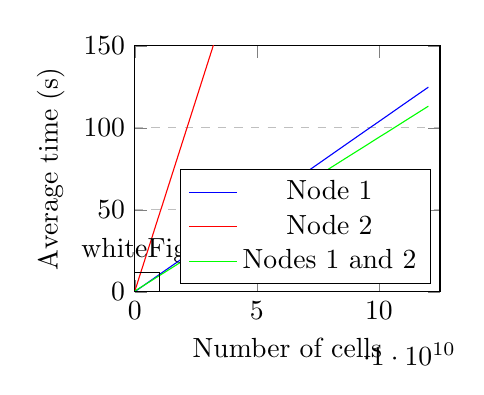
\begin{tikzpicture}
\begin{axis}[
    %title={Average time to compute edit distance},
    xlabel={Number of cells},
    ylabel={Average time (s)},
    xmin=0, xmax=125000000000,
    ymin=0, ymax=150,
    legend pos=south east,
    ymajorgrids=true,
    grid style=dashed,
    scaled x ticks={real:10000000000},
    width=0.45\linewidth,
]


\addplot[
    color=blue,
    smooth,
    ]
    coordinates {
    (16777216, 0.09921685714285713)(33554432, 0.12080128571428571)(67108864, 0.160687)(134217728, 0.2424785714285714)(268435456, 0.38340228571428575)(536870912, 0.6664877142857142)(1000000000, 1.152977142857143)(1500000000, 1.6785985714285712)(2147483648, 2.357917142857143)(3000000000, 3.2444357142857143)(4294967296, 4.582278571428572)(6000000000, 6.368568571428573)(7000000000, 7.4005728571428575)(8589934592, 9.062895000000001)(10000000000, 10.52197142857143)(11000000000, 11.564114285714284)(12000000000, 12.593114285714284)(13000000000, 13.643714285714285)(14000000000, 14.677214285714285)(17179869184, 17.97048571428571)(25769803776, 26.88624285714286)(34359738368, 35.8241)(42949672960, 44.70372857142858)(51539607552, 53.59438571428571)(60129542144, 62.536071428571425)(68719476736, 71.40738571428571)(77309411328, 80.32997142857143)(85899345920, 89.26152857142857)(94489280512, 98.17172857142855)(100000000000, 103.8337142857143)(103079215104, 107.02371428571429)(111669149696, 115.95128571428572)(120259084288, 124.80914285714286)
    };

\addplot[
    color=red,
    smooth,
    ]
    coordinates {
    (16777216, 0.5445155714285714)(33554432, 0.626533)(67108864, 0.8027252857142858)(134217728, 1.12474)(268435456, 1.7438942857142856)(536870912, 3.0209571428571427)(1000000000, 5.162437142857143)(1500000000, 7.543924285714286)(2147483648, 10.5999)(3000000000, 14.472014285714282)(4294967296, 20.55514285714286)(6000000000, 28.49077142857143)(7000000000, 33.10725714285714)(8589934592, 40.61537142857143)(10000000000, 47.16012857142857)(11000000000, 51.74827142857142)(12000000000, 56.35255714285715)(13000000000, 61.09289999999999)(14000000000, 65.73704285714287)(17179869184, 80.55284285714286)(25769803776, 120.55142857142857)(34359738368, 160.5607142857143)(42949672960, 200.45)(51539607552, 240.47842857142857)(60129542144, 280.283)(68719476736, 320.3165714285714)(77309411328, 360.40957142857144)(85899345920, 400.24628571428576)(94489280512, 440.2641428571429)(100000000000, 465.98900000000003)(103079215104, 480.2848571428571)(111669149696, 520.3457142857143)(120259084288, 560.304)
    };

\addplot[
    color=green,
    smooth,
    ]
    coordinates {
    (16777216, 0.496333)(33554432, 0.5080268571428571)(67108864, 0.6234567142857143)(134217728, 0.6975642857142856)(268435456, 0.7566615714285714)(536870912, 1.0175524285714288)(1000000000, 1.4202885714285713)(1500000000, 1.9164114285714287)(2147483648, 2.5176842857142856)(3000000000, 3.249014285714286)(4294967296, 4.516901428571428)(6000000000, 6.0832242857142855)(7000000000, 7.0254957142857135)(8589934592, 8.529228)(10000000000, 9.85383)(11000000000, 10.788914285714286)(12000000000, 11.679885714285714)(13000000000, 12.648942857142856)(14000000000, 13.559485714285714)(17179869184, 16.574385714285714)(25769803776, 24.604942857142856)(34359738368, 32.70814285714285)(42949672960, 40.747)(51539607552, 48.7744)(60129542144, 56.66547142857142)(68719476736, 64.66221428571428)(77309411328, 72.89688571428572)(85899345920, 81.01222857142857)(94489280512, 89.02959999999999)(100000000000, 94.25682857142858)(103079215104, 97.06402857142858)(111669149696, 105.15614285714285)(120259084288, 113.20742857142857)
    };

\addplot[
    color=black,
    mark=none,
] coordinates {(0,0) (0,12) (10000000000,12) (10000000000,0) (0,0)};

\pgfplotsset{
    after end axis/.code={
        \node[above] at (axis cs:10000000000,12){\contour{white}{Fig. \ref{result_graph_zoom}}};
    }
}


\legend{Node 1, Node 2, Nodes 1 and 2}
\end{axis}
\end{tikzpicture}
}
    \hspace{0.05\linewidth}
    \subfloat[][Zoomed in]{\label{result_graph_zoom}
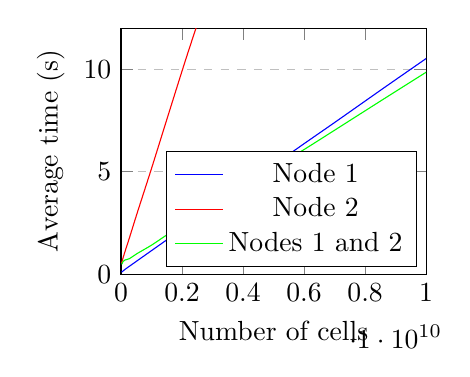
\begin{tikzpicture}
\begin{axis}[
    %title={Average time to compute edit distance},
    xlabel={Number of cells},
    ylabel={Average time (s)},
    xmin=0, xmax=10000000000,
    ymin=0, ymax=12,
    legend pos=south east,
    ymajorgrids=true,
    grid style=dashed,
    scaled x ticks={real:10000000000},
    width=0.45\linewidth,
]


\addplot[
    color=blue,
    smooth,
    ]
    coordinates {
    (16777216, 0.09921685714285713)(33554432, 0.12080128571428571)(67108864, 0.160687)(134217728, 0.2424785714285714)(268435456, 0.38340228571428575)(536870912, 0.6664877142857142)(1000000000, 1.152977142857143)(1500000000, 1.6785985714285712)(2147483648, 2.357917142857143)(3000000000, 3.2444357142857143)(4294967296, 4.582278571428572)(6000000000, 6.368568571428573)(7000000000, 7.4005728571428575)(8589934592, 9.062895000000001)(10000000000, 10.52197142857143)(11000000000, 11.564114285714284)(12000000000, 12.593114285714284)(13000000000, 13.643714285714285)(14000000000, 14.677214285714285)(17179869184, 17.97048571428571)(25769803776, 26.88624285714286)(34359738368, 35.8241)(42949672960, 44.70372857142858)(51539607552, 53.59438571428571)(60129542144, 62.536071428571425)(68719476736, 71.40738571428571)(77309411328, 80.32997142857143)(85899345920, 89.26152857142857)(94489280512, 98.17172857142855)(100000000000, 103.8337142857143)(103079215104, 107.02371428571429)(111669149696, 115.95128571428572)(120259084288, 124.80914285714286)
    };

\addplot[
    color=red,
    smooth,
    ]
    coordinates {
    (16777216, 0.5445155714285714)(33554432, 0.626533)(67108864, 0.8027252857142858)(134217728, 1.12474)(268435456, 1.7438942857142856)(536870912, 3.0209571428571427)(1000000000, 5.162437142857143)(1500000000, 7.543924285714286)(2147483648, 10.5999)(3000000000, 14.472014285714282)(4294967296, 20.55514285714286)(6000000000, 28.49077142857143)(7000000000, 33.10725714285714)(8589934592, 40.61537142857143)(10000000000, 47.16012857142857)(11000000000, 51.74827142857142)(12000000000, 56.35255714285715)(13000000000, 61.09289999999999)(14000000000, 65.73704285714287)(17179869184, 80.55284285714286)(25769803776, 120.55142857142857)(34359738368, 160.5607142857143)(42949672960, 200.45)(51539607552, 240.47842857142857)(60129542144, 280.283)(68719476736, 320.3165714285714)(77309411328, 360.40957142857144)(85899345920, 400.24628571428576)(94489280512, 440.2641428571429)(100000000000, 465.98900000000003)(103079215104, 480.2848571428571)(111669149696, 520.3457142857143)(120259084288, 560.304)
    };

\addplot[
    color=green,
    smooth,
    ]
    coordinates {
    (16777216, 0.496333)(33554432, 0.5080268571428571)(67108864, 0.6234567142857143)(134217728, 0.6975642857142856)(268435456, 0.7566615714285714)(536870912, 1.0175524285714288)(1000000000, 1.4202885714285713)(1500000000, 1.9164114285714287)(2147483648, 2.5176842857142856)(3000000000, 3.249014285714286)(4294967296, 4.516901428571428)(6000000000, 6.0832242857142855)(7000000000, 7.0254957142857135)(8589934592, 8.529228)(10000000000, 9.85383)(11000000000, 10.788914285714286)(12000000000, 11.679885714285714)(13000000000, 12.648942857142856)(14000000000, 13.559485714285714)(17179869184, 16.574385714285714)(25769803776, 24.604942857142856)(34359738368, 32.70814285714285)(42949672960, 40.747)(51539607552, 48.7744)(60129542144, 56.66547142857142)(68719476736, 64.66221428571428)(77309411328, 72.89688571428572)(85899345920, 81.01222857142857)(94489280512, 89.02959999999999)(100000000000, 94.25682857142858)(103079215104, 97.06402857142858)(111669149696, 105.15614285714285)(120259084288, 113.20742857142857)
    };


\legend{Node 1, Node 2, Nodes 1 and 2}
\end{axis}
\end{tikzpicture}
}
    \caption{Average time to compute edit distance} \label{result_graph_total}
    %\floatpagefraction
%\end{figure*}
\vspace*{\floatsep}
%\begin{figure*}[h]
    \centering
    \subfloat[][Overview]{\label{result_graph_cell}
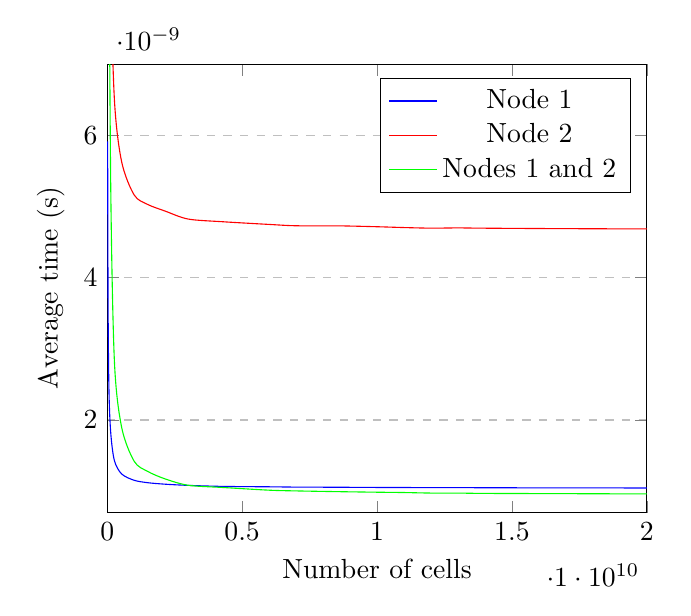
\begin{tikzpicture}
\begin{axis}[
    %title={Average time per cell},
    xlabel={Number of cells},
    ylabel={Average time (s)},
    xmin=0, xmax=20000000000,
    ymin=7e-10, ymax=7e-09,
    legend pos=north east,
    ymajorgrids=true,
    grid style=dashed,
    scaled x ticks={real:10000000000},
]


\addplot[
    color=blue,
    smooth,
    ]
    coordinates {
    (16777216, 5.9137855257306775e-09)(33554432, 3.600158861705235e-09)(67108864, 2.3944228887557983e-09)(134217728, 1.8066061394555226e-09)(268435456, 1.4282848153795516e-09)(536870912, 1.2414301080363135e-09)(1000000000, 1.152977142857143e-09)(1500000000, 1.119065714285714e-09)(2147483648, 1.0979907321078438e-09)(3000000000, 1.0814785714285714e-09)(4294967296, 1.0668948691870486e-09)(6000000000, 1.0614280952380955e-09)(7000000000, 1.057224693877551e-09)(8589934592, 1.0550598381087185e-09)(10000000000, 1.0521971428571429e-09)(11000000000, 1.0512831168831168e-09)(12000000000, 1.0494261904761902e-09)(13000000000, 1.0495164835164835e-09)(14000000000, 1.0483724489795918e-09)(17179869184, 1.0460199389074528e-09)(25769803776, 1.0433235383104711e-09)(34359738368, 1.042618532665074e-09)(42949672960, 1.0408397897013597e-09)(51539607552, 1.0398679435075748e-09)(60129542144, 1.0400224115927607e-09)(68719476736, 1.0391142235935798e-09)(77309411328, 1.0390710529117357e-09)(85899345920, 1.0391409575406993e-09)(94489280512, 1.0389721250863041e-09)(100000000000, 1.0383371428571429e-09)(103079215104, 1.0382666784737793e-09)(111669149696, 1.038346634051957e-09)(120259084288, 1.0378354666184407e-09)
    };

\addplot[
    color=red,
    smooth,
    ]
    coordinates {
    (16777216, 3.245565720966884e-08)(33554432, 1.8672138452529907e-08)(67108864, 1.1961538876805988e-08)(134217728, 8.379966020584107e-09)(268435456, 6.4965124641145975e-09)(536870912, 5.626971168177468e-09)(1000000000, 5.162437142857143e-09)(1500000000, 5.029282857142857e-09)(2147483648, 4.935963079333305e-09)(3000000000, 4.824004761904761e-09)(4294967296, 4.785867141825813e-09)(6000000000, 4.748461904761905e-09)(7000000000, 4.729608163265305e-09)(8589934592, 4.728251535977636e-09)(10000000000, 4.7160128571428574e-09)(11000000000, 4.704388311688311e-09)(12000000000, 4.696046428571429e-09)(13000000000, 4.699453846153845e-09)(14000000000, 4.695503061224491e-09)(17179869184, 4.688792562644397e-09)(25769803776, 4.678011117946534e-09)(34359738368, 4.6729318065834904e-09)(42949672960, 4.667090252041816e-09)(51539607552, 4.665895609096402e-09)(60129542144, 4.661319378231253e-09)(68719476736, 4.661219593669687e-09)(77309411328, 4.661910694151644e-09)(85899345920, 4.659480016146388e-09)(94489280512, 4.6594083526885355e-09)(100000000000, 4.6598900000000005e-09)(103079215104, 4.659376351074094e-09)(111669149696, 4.6597087530644385e-09)(120259084288, 4.659140748637063e-09)
    };

\addplot[
    color=green,
    smooth,
    ]
    coordinates {
    (16777216, 2.9583752155303957e-08)(33554432, 1.514038017817906e-08)(67108864, 9.290228996958051e-09)(134217728, 5.197258932249886e-09)(268435456, 2.8187840112618036e-09)(536870912, 1.8953390951667517e-09)(1000000000, 1.4202885714285714e-09)(1500000000, 1.277607619047619e-09)(2147483648, 1.1723881055201802e-09)(3000000000, 1.083004761904762e-09)(4294967296, 1.0516730669353688e-09)(6000000000, 1.0138707142857144e-09)(7000000000, 1.003642244897959e-09)(8589934592, 9.929328225553036e-10)(10000000000, 9.85383e-10)(11000000000, 9.808103896103896e-10)(12000000000, 9.733238095238094e-10)(13000000000, 9.729956043956044e-10)(14000000000, 9.68534693877551e-10)(17179869184, 9.647562235061612e-10)(25769803776, 9.547974470825421e-10)(34359738368, 9.519322442689111e-10)(42949672960, 9.487150236964226e-10)(51539607552, 9.463479121526082e-10)(60129542144, 9.423898704045889e-10)(68719476736, 9.409590607642063e-10)(77309411328, 9.429238234010953e-10)(85899345920, 9.43106466106006e-10)(94489280512, 9.422190487384794e-10)(100000000000, 9.425682857142859e-10)(103079215104, 9.416450103301378e-10)(111669149696, 9.416758625225706e-10)(120259084288, 9.41362802167328e-10)
    };


\legend{Node 1, Node 2, Nodes 1 and 2}
\end{axis}
\end{tikzpicture}
}
    \hspace{0.05\linewidth}
    \subfloat[][Zoomed in]{\label{result_graph_cell_zoom}
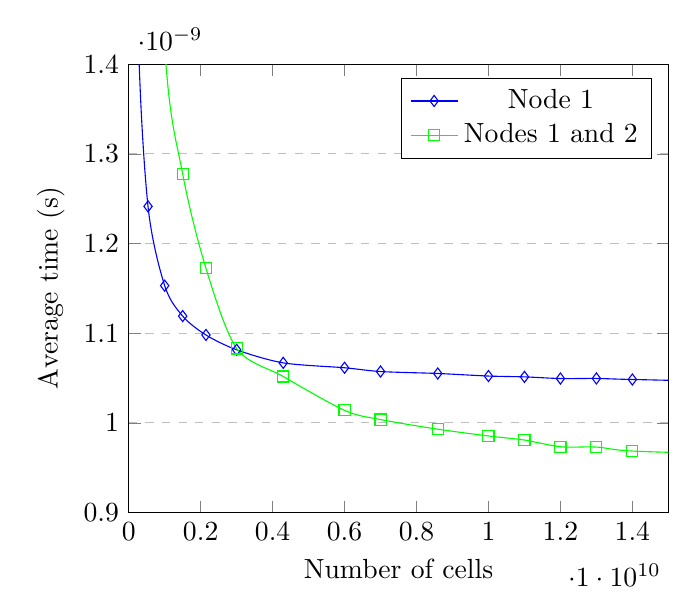
\begin{tikzpicture}
\begin{axis}[
    %title={Average time per cell},
    xlabel={Number of cells},
    ylabel={Average time (s)},
    xmin=0, xmax=15000000000,
    ymin=9e-10, ymax=1.4e-09,
    legend pos=north east,
    ymajorgrids=true,
    grid style=dashed,
    scaled x ticks={real:10000000000},
]


\addplot[
    color=blue,
    smooth,mark=diamond,
    ]
    coordinates {
    (16777216, 5.9137855257306775e-09)(33554432, 3.600158861705235e-09)(67108864, 2.3944228887557983e-09)(134217728, 1.8066061394555226e-09)(268435456, 1.4282848153795516e-09)(536870912, 1.2414301080363135e-09)(1000000000, 1.152977142857143e-09)(1500000000, 1.119065714285714e-09)(2147483648, 1.0979907321078438e-09)(3000000000, 1.0814785714285714e-09)(4294967296, 1.0668948691870486e-09)(6000000000, 1.0614280952380955e-09)(7000000000, 1.057224693877551e-09)(8589934592, 1.0550598381087185e-09)(10000000000, 1.0521971428571429e-09)(11000000000, 1.0512831168831168e-09)(12000000000, 1.0494261904761902e-09)(13000000000, 1.0495164835164835e-09)(14000000000, 1.0483724489795918e-09)(17179869184, 1.0460199389074528e-09)(25769803776, 1.0433235383104711e-09)(34359738368, 1.042618532665074e-09)(42949672960, 1.0408397897013597e-09)(51539607552, 1.0398679435075748e-09)(60129542144, 1.0400224115927607e-09)(68719476736, 1.0391142235935798e-09)(77309411328, 1.0390710529117357e-09)(85899345920, 1.0391409575406993e-09)(94489280512, 1.0389721250863041e-09)(100000000000, 1.0383371428571429e-09)(103079215104, 1.0382666784737793e-09)(111669149696, 1.038346634051957e-09)(120259084288, 1.0378354666184407e-09)
    };

\addplot[
    color=green,
    smooth,mark=square,
    ]
    coordinates {
    (16777216, 2.9583752155303957e-08)(33554432, 1.514038017817906e-08)(67108864, 9.290228996958051e-09)(134217728, 5.197258932249886e-09)(268435456, 2.8187840112618036e-09)(536870912, 1.8953390951667517e-09)(1000000000, 1.4202885714285714e-09)(1500000000, 1.277607619047619e-09)(2147483648, 1.1723881055201802e-09)(3000000000, 1.083004761904762e-09)(4294967296, 1.0516730669353688e-09)(6000000000, 1.0138707142857144e-09)(7000000000, 1.003642244897959e-09)(8589934592, 9.929328225553036e-10)(10000000000, 9.85383e-10)(11000000000, 9.808103896103896e-10)(12000000000, 9.733238095238094e-10)(13000000000, 9.729956043956044e-10)(14000000000, 9.68534693877551e-10)(17179869184, 9.647562235061612e-10)(25769803776, 9.547974470825421e-10)(34359738368, 9.519322442689111e-10)(42949672960, 9.487150236964226e-10)(51539607552, 9.463479121526082e-10)(60129542144, 9.423898704045889e-10)(68719476736, 9.409590607642063e-10)(77309411328, 9.429238234010953e-10)(85899345920, 9.43106466106006e-10)(94489280512, 9.422190487384794e-10)(100000000000, 9.425682857142859e-10)(103079215104, 9.416450103301378e-10)(111669149696, 9.416758625225706e-10)(120259084288, 9.41362802167328e-10)
    };


\legend{Node 1, Nodes 1 and 2}
\end{axis}
\end{tikzpicture}
}
    \caption{Average time per cell} \label{result_graph_cell_total}
\end{figure*}


\subsection{MPI Algorithm \ref*{MPIalg}} \label{ver:MPIalg}
As the nodes in a cluster only communicate the right most columns of blocks, no concurrent variable manipulation can occur.
Therefore, permission-based separation logic is not required for this algorithm.
There are no circular dependencies, so no deadlocks can occur.
This cuts down the need for verification even further, leaving only trivial \textit{requires} and \textit{ensures} statements.

\subsection{Verification with VerCors} \label{ver:vercors}
Unfortunately, OpenCL is not sufficiently supported by VerCors to do automatic verification.
Rewriting the kernel in PVL, the native language of VerCors, does not help, as there is no support for kernel arguments.
In further research support could be built into VerCors, but in the mean time the manual verification provided in \crefrange{block}{MPIalg} will have to do.


\section{Testing the performance of the implementation}


\begin{comment}
\section{Expected results}
As only the answer of subquestion 4 will consist of tests only the expected results of these tests will be discussed.
When comparing different cluster sizes, and lengths of data, the time required to compute the edit distance can be used to define most efficient setup.
For each cluster size and data length the computation time can be divided in four ranges.

The first range is a negative time difference, which indicates the use of MPI, dividing the algorithm, or the use of a cluster in general is inefficient.

The next range is a difference almost equal to zero, which indicates that dividing the calculation gives too much overhead, denying any reduction of the processing time required.

The third range is a difference up to $n$ times as fast as the single node implementation, where $n$ is the number of nodes in the cluster.
This would mean that dividing the computation over a cluster is more efficient than calculating it on a single node, but that the overhead caused by the distribution of the algorithm impacts the performance.
The distribution of algorithms over a GPU-cluster have already shown improved performances, so I suspect to have some setups to be within this range.

The last range is the most improbable. It ranges from $n$ times as fast to beyond, where $n$ is the number of nodes.
This would mean that the algorithm is more efficient as it is divided on multiple computers.
If, for example, the number of nodes is doubled the speed would more than double.
This would be strange since the processing power does not double.

To compare the efficiency an implementation resolving the edit distance problem has to be made. This will be done according to the schedule mentioned in table \ref{schedule}.

\section{Related work}
\subsection{Edit distance problem on GPU}
As mentioned before the edit distance problem has already been implemented on a single GPU \cite{Heus:GPGPU}.
This implementation also uses the operations insert, delete, and replace.
This implementation will be improved if necessary and will probably be the base of the future implementation.
The result of this project could be compared to this single node implementation to calculate the difference in time required to compute the edit distance of two strings.

%\balancecolumns
\subsection{Benchmark on a GPU-cluster}
This is an MPI-OpenCL implementation of the LINPACK benchmark which was run on a cluster containing 49 nodes, each node containing two eight-core CPUs and four GPUs \cite{Cluster}.
The implementation achieves 93.69 Tflops, which is 46 percent of the theoretical peak.
It shows a successful implementation of MPI in combination with OpenCL, which is required in the future implementation of the edit distance algorithm.

\section{Research schedule}
The research schedule for this paper is given in Table \ref{schedule}.

\begin{table}
\centering \caption{Research schedule} \label{schedule}
\begin{tabular}{|l|l|} \hline
\textbf{Deadline} & \textbf{Task/Deliverable}       \\ \hline
Oct 12 & Peer reviews                               \\ \hline
Oct 21 & Final proposal                             \\ \hline
Oct 26 & (No) Go                                    \\ \hline
Nov 2  & Research                                   \\ \hline
Nov 16 & Dividing the algorithm and implementing    \\ \hline
Nov 23 & Researching MPI                            \\ \hline
Nov 30 & Implementing MPI                           \\ \hline
Dec 7  & Verifying the implementation               \\ \hline
Dec 14 & Optimizing and debugging                   \\ \hline
Dec 18 & Getting a test environment                 \\ \hline
Jan 11 & Writing the paper                          \\ \hline
Jan 18 & Writing a presentation                     \\ \hline
\end{tabular}
\end{table}
\end{comment}

%\balancecolumns
\bibliographystyle{abbrv}
\bibliography{sigproc}


\end{document}
